\section{Scheduler subsystem}

%%%%%%%%%%%%%%%%%%%%%%%%%%%%%%%%%%%%%%%%%%%%%%%%%%%%%%%%%%%
%
% SUBSECTION: Overview of scheduler internals & integration
%
%%%%%%%%%%%%%%%%%%%%%%%%%%%%%%%%%%%%%%%%%%%%%%%%%%%%%%%%%%%
\subsection{Overview of scheduler internals \& integration}
    
\begin{frame}{Linux scheduling overview}    
    \begin{itemize}
        \item Linux has a modular scheduler architecture \pause
        \item Allows different scheduling policies to co-exist \pause
        \item Policies are wrapped up in so-called scheduler classes \pause
        \item Implementing a new scheduling policy for Linux mainly consists of writing a new scheduler class
    \end{itemize}
\end{frame}

\begin{frame}{Linux scheduling overview (2)}    
    \begin{itemize}
        \item There are 2 main scheduling classes \pause
        \item Real-Time scheduling class is responsible for \texttt{SCHED\_FIFO} \& \texttt{SCHED\_RR} policies \pause
        \item Completely Fair Scheduler --- for \texttt{SCHED\_NORMAL} \& \texttt{SCHED\_BATCH} policies \pause
        \item Newly created processes are assigned the normal scheduling policy \pause
        \item All forked subprocesses will inherit it
    \end{itemize}
\end{frame}

% \begin{frame}{Linux scheduling overview (3)}
%     \missingfigure{A picture of VCPU with shares, aligned on a superperiod proportional to their share}
% \end{frame}

\begin{frame}{Superperiod}
    \begin{itemize}
        \item Starts when there is at least one task \pause
        \item Schedules tasks from the \texttt{eligible\_q}
        \item Preempted tasks return to \texttt{waiting\_q}\pause
        \item \textit{Idle} period begins when the \texttt{eligible\_q} is empty
    \end{itemize}
\end{frame}

% \dummyslide[vcpus]

\begin{frame}{Idle period}
    \begin{itemize}
        \item When the \texttt{eligible\_q} is empty, our scheduler ``steals'' the \textit{idle} task
        \item This happens only if the superperiod has extra time left\pause
        \item Idle task is scheduled until the end of superperiod
    \end{itemize}
\end{frame}


\begin{frame}[fragile]{Restart of period}
    \begin{itemize}
        \item When the superperiod is finished, the \texttt{eligible\_q} and \texttt{waiting\_q} are swapped
        \item Precisely speaking, special pointer variables are swapped:
            \begin{lstlisting}[language=C,gobble=12]
            tmp = rq->ospj.ptr_waiting_q;
            rq->ospj.ptr_waiting_q = rq->ospj.ptr_eligible_q;
            rq->ospj.ptr_eligible_q = tmp;
            \end{lstlisting} 
        \item Time is then replenished by \texttt{replenish\_super\_period()}
    \end{itemize}
\end{frame}

\begin{frame}{Integrating a scheduler}

{
    With kernel:
    \begin{enumerate}
        \item Struct declarations
        \item Config flags
        \item Scheduler list
    \end{enumerate}
}\pause 

{
    With userspace:
    \begin{enumerate}
        \item Syscall
        \item Userspace tool
    \end{enumerate}
}\pause

{
    With power-saving code:
    \begin{enumerate}
         \item Changing the \texttt{sched\_class} of idle task
         \item Calling the power-related code inside \texttt{idle.c}
    \end{enumerate}
}
\end{frame}

%%%%%%%%%%%%%%%%%%%%%%%%%%%%%%%%%%%%%%%%%%%%%%%%%%%%%%%%%%%
%
% SUBSECTION: Integration with kernel
%
%%%%%%%%%%%%%%%%%%%%%%%%%%%%%%%%%%%%%%%%%%%%%%%%%%%%%%%%%%%
\subsection{Integration with kernel}

\begin{frame}{Custom runqueue}
    \begin{itemize}
        \item Each scheduling class has its runqueue structure \pause
        \item Main runqueue has a field for each scheduling class \pause
        \item The is one (main) runqueue per CPU
    \end{itemize}
\end{frame}

% TODO firstnumber 365
\begin{frame}[fragile]{Custom runqueue: \texttt{struct ospj\_rq}}
\begin{lstlisting}[
language=C,
gobble=0,
linebackgroundcolor={%
    \btLstHL<1>{5,6}%   two queues
    \btLstHL<2>{3,4}%   their pointers
    \btLstHL<3>{7}%     pointer backwards
    \btLstHL<4>{8}%     stealing the idle
    \btLstHL<5>{10}%    stealing request
    \btLstHL<6>{11}%    ticks left in the superperiod
}]
struct ospj_rq {
    struct list_head ospj_list_head;
    struct list_head *ptr_eligible_q;
    struct list_head *ptr_waiting_q;
    struct list_head eligible_q;
    struct list_head waiting_q;
    struct rq *rq;
    struct task_struct *idle;
    unsigned int nr_running;
    unsigned int idle_request;
    unsigned int period_ticks;
};
\end{lstlisting}
\end{frame}

\begin{frame}[fragile]{Main runqueue: \texttt{struct rq}}
\begin{lstlisting}[
language=C,
basicstyle=\small\ttfamily,
gobble=0,
firstnumber=417,
linebackgroundcolor={%
    \btLstHL<1>{422}%
    \btLstHL<2>{421}%
}]
struct rq {
    ...
    struct cfs_rq cfs;
    struct rt_rq rt;
#ifdef CONFIG_SCHED_VMS
    struct ospj_rq ospj;
#endif /* CONFIG_SCHED_VMS */
    ...
}
\end{lstlisting}
\end{frame}


\begin{frame}[fragile]{Task structure}
\pnote{Each task in the system is assigned to a particular scheduling class}
\begin{lstlisting}[
language=C,
basicstyle=\small\ttfamily,
% basicstyle=\footnotesize\ttfamily,
gobble=0,
firstnumber=1055,
linebackgroundcolor={%
    \btLstHL<1>{1065,1057}%
    \btLstHL<2>{1060,1062}%
    \btLstHL<3>{1061}%
}]
struct task_struct {
    ...
    const struct sched_class *sched_class;
    ...
#ifdef CONFIG_SCHED_VMS
    unsigned int share;
    unsigned int ospj_time_slice;
    unsigned int ospj_assigned_time_slice;
#endif /* CONFIG_SCHED_VMS */
    ...
    unsigned int policy;
    ...
}
\end{lstlisting}
\end{frame}

\begin{frame}{Configuration options}
    \begin{itemize}
        \item All this code must be integrated into kernel
        \item The integration must be seamless
        \item We used the configuration option declared in \texttt{Kconfig}
    \end{itemize}
\end{frame}

\begin{frame}[fragile]{Configuration options (2)}
    \begin{lstlisting}[language=C,
    gobble=4,
    language=ruby,
    firstnumber=2334,
    linebackgroundcolor={%
        \btLstHL<1>{2334,2340}%
        \btLstHL<2>{2337}%
        \btLstHL<3>{2338}%
        \btLstHL<4>{2336}%
    }
]
    menu "VMS scheduler (OSPJ)"
    
    config SCHED_VMS
        bool "Virtual Machines Scheduling (VMS) policy"
        default y

    endmenu
    \end{lstlisting}
\end{frame}

\begin{frame}{Configuration options (3)}
    \begin{figure}
       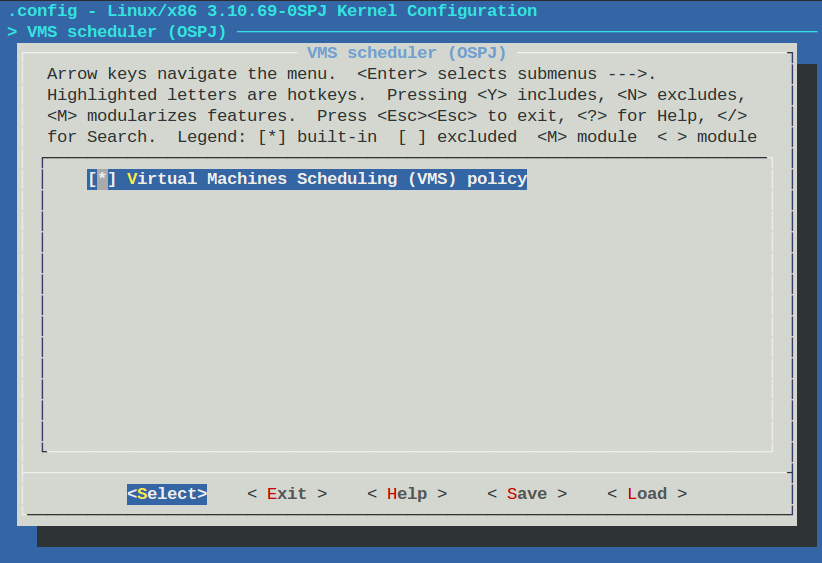
\includegraphics[width=0.8\linewidth]{img/menuconfig.png}
    \end{figure}
\end{frame}


%%%%%%%%%%%%%%%%%%%%%%%%%%%%%%%%%%%%%%%%%%%%%%%%%%%%%%%%%%%
%
% SUBSECTION: Integration with userspace
%
%%%%%%%%%%%%%%%%%%%%%%%%%%%%%%%%%%%%%%%%%%%%%%%%%%%%%%%%%%%

\subsection{Integration with userspace}

\begin{frame}{\texttt{sched\_setscheduler(2)} syscall}
    \begin{itemize}
        \item Used to set the scheduler and priority
        \item Validates parameters before making changes
        \item We extended it to handle \texttt{SCHED\_VMS} policy
        \item And accept the \texttt{share} parameter
    \end{itemize}
\end{frame}

\begin{frame}[fragile]{\texttt{struct sched\_param}}
\begin{lstlisting}[language=C,linebackgroundcolor={%
        \btLstHL<1>{4}%
    }]
struct sched_param {
    int sched_priority;
#ifdef CONFIG_SCHED_VMS
    unsigned int share;
#endif /* CONFIG_SCHED_VMS */
};
\end{lstlisting}
\end{frame}

\begin{frame}{Userspace headers}
    \begin{itemize}
        \item Required by the userspace tools at the compilation phase
        \item Must match the installed kernel
        \item Automatically installed on \texttt{deneb} with DevOps help on each build
        \item Main file changes to \texttt{/usr/include/linux/sched.h}
    \end{itemize}
\end{frame}

\begin{frame}[fragile]{Userspace headers (2)}

Typical use case:

\begin{lstlisting}[language=C]
#ifdef SCHED_VMS
    vms_support = "ENABLED";
#else
    vms_support = "DISABLED";
#endif
\end{lstlisting}
\end{frame}

\begin{frame}{All together: {\ttfamily\bfseries ospj-setsched} tool}
    \begin{itemize}
        \item Designed to \textbf{change} and \textbf{retrieve} the scheduling policies
        \item Allows to set the {\bfseries {\ttfamily SCHED\_VMS}} policy
        \item Allows to supply the {\bfseries task {\itshape share}} (for OSPJ scheduler)
    \end{itemize}
\end{frame}

\begin{frame}{Changing policy for QEMU threads}
    \begin{itemize}
        \item Is main design target of the \texttt{ospj-setsched} tool
        \item Minimally, only change the policy for the threads corresponding to the VCPUs
        \item Also, possible to schedule other threads:
        \begin{itemize}
            \item Configuration dependent threads
            \item Worker threads
            \item Dedicated threads
            \item Reusable threads 
        \end{itemize}
    \end{itemize}
\end{frame}


\subsection{Evaluation}

\begin{frame}{Scheduler fairness measurement}
    \begin{enumerate}
        \item Calculate $N$th element of the Fibonacci series
        \item Time it inside QEMU
        \item \texttt{time fibo 10,000,000 > /dev/null}
    \end{enumerate}
\end{frame}

\begin{frame}{Scheduler fairness measurement results}
    \begin{figure}
       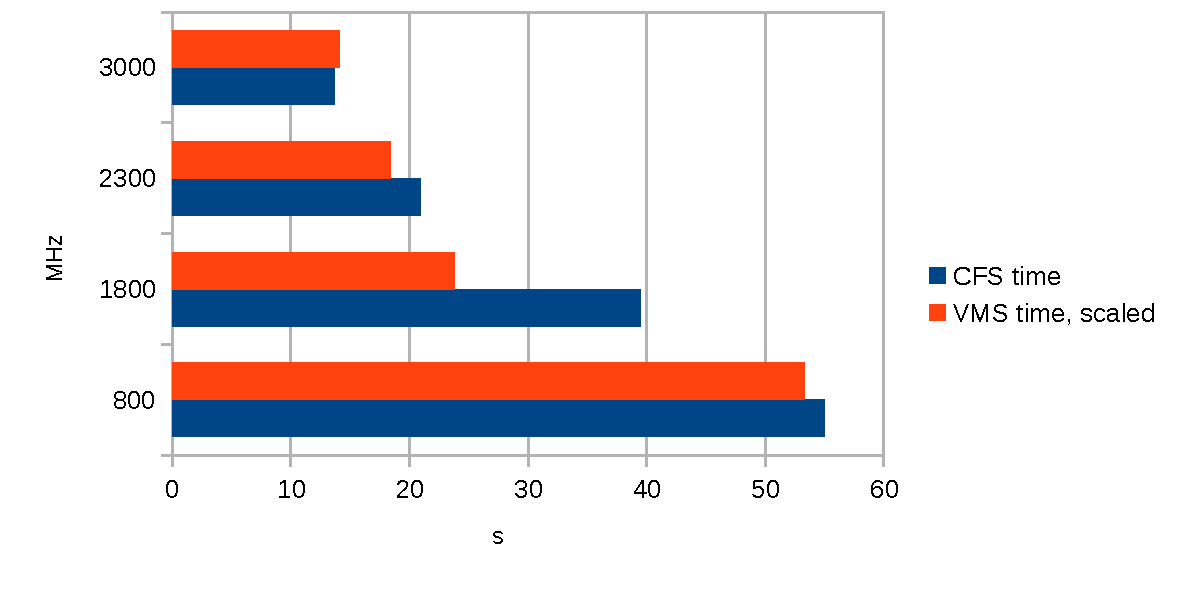
\includegraphics[width=1\linewidth]{img/fibo.pdf}
    \end{figure}
\end{frame}
